\section{Arrivée sur la plateforme}
\label{sec:arrivee}

La page d’accueil est une page essentielle de la plateforme. Elle doit être claire et précise car elle présente à l’utilisateur le site web.
Lorsque l’utilisateur arrive sur la plateforme, il lui est proposé plusieurs onglets aux fonctionnalités diverses : la recherche (articles, journaux, revue de presse), la proposition de journaux/articles et la connexion/inscription à la plateforme.

\subsection{La recherche dans la base (articles, journaux)}
\label{sec:arrivee_recherche}
L’utilisateur ici a accès à un moteur de recherche assez classique qui propose des filtres tels que : le titre, le thème, la période, le journal, la région. L’utilisateur peut également effectuer une recherche plein texte dans la base de journaux. L’affichage des résultats se fera sous forme de liste incluant le titre, la date, et le nom de journal. Dans le cas d’une recherche plein texte, il sera également affiché dans les résultats un extrait de l’article où les mots clés ont été trouvés. L’utilisateur peut ensuite trier les résultats obtenus en fonction de la date, des ajouts récents, des plus visités. Une fois l’article trouvé, l’utilisateur peut donc passer à la visualisation du document décrite dans une autre section de ce rapport.

\subsection{La recherche d’une revue de presse}
\label{sec:arrivee_revue}
En cliquant sur cet onglet, l’utilisateur accède aussi à un moteur de recherche concernant uniquement les revues de presse. Les critères de recherche sont essentiellement le thème, la date, l’événement. L’affichage se fait aussi sous forme d’une liste présentant le thème et la date des revues de presse. Il sera également possible de trier les résultats selon les mêmes critères que ceux énoncés pour la recherche dans la base.

\subsection{La proposition d’articles}
\label{sec:arrivee_article}
Nous avons trouvé intéressant de proposer à l'utilisateur des éléments dès sont arrivée sur la plateforme. Ainsi, sur la page d’accueil, l’utilisateur pourra consulter des petits onglets avec des propositions sur les articles les plus consultés, les articles récemment ajoutés, la dernière revue de presse créée,…

\subsection{Création/connexion à un compte utilisateur}
\label{sec:arrivee_utilisateur}
L’utilisateur peut en cliquant ici créer son compte utilisateur ou se connecter.

    \begin{figure}[H]
        \centering
        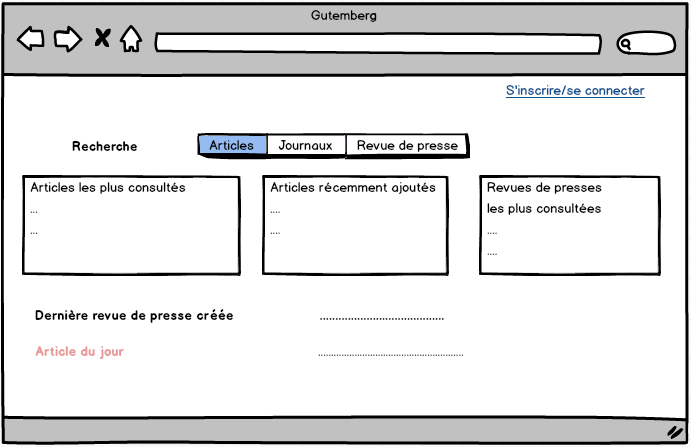
\includegraphics[width=\textwidth]{figures/Accueil.png}
            \caption{Page d'accueil de la plateforme}
            \label{fig:accueil}
    \end{figure}